%; whizzy chapter
% -initex iniptex -latex platex -format platex -bibtex jbibtex -fmt fmt
% 以上 whizzytex を使用する場合の設定。


%     Tokyo Debian Meeting resources
%     Copyright (C) 2008 Junichi Uekawa

%     This program is free software; you can redistribute it and/or modify
%     it under the terms of the GNU General Public License as published by
%     the Free Software Foundation; either version 2 of the License, or
%     (at your option) any later version.

%     This program is distributed in the hope that it will be useful,
%     but WITHOUT ANY WARRANTY; without even the implied warranty of
%     MERCHANTABILITY or FITNESS FOR A PARTICULAR PURPOSE.  See the
%     GNU General Public License for more details.

%     You should have received a copy of the GNU General Public License
%     along with this program; if not, write to the Free Software
%     Foundation, Inc., 51 Franklin St, Fifth Floor, Boston, MA  02110-1301 USA

%  preview (shell-command (concat "evince " (replace-regexp-in-string "tex$" "pdf"(buffer-file-name)) "&"))
% 画像ファイルを処理するためにはebbを利用してboundingboxを作成。
%(shell-command "cd image200804; ebb *.png")

%%ここからヘッダ開始。

\documentclass[mingoth,a4paper]{jsarticle}
\usepackage{monthlyreport}

% 日付を定義する、毎月変わります。
\newcommand{\debmtgyear}{2008}
\newcommand{\debmtgmonth}{4}
\newcommand{\debmtgdate}{19}
\newcommand{\debmtgnumber}{39}

\begin{document}

\begin{titlepage}
\thispagestyle{empty}

% タイトルページ:編集必要な部分は最初のマクロに飛ばすこと

\vspace*{-2cm}
第\debmtgnumber{}回 東京エリア Debian 勉強会資料

\hspace*{-2.4cm}
\includegraphics[width=210mm]{image200801/2008title.eps}\\
\hfill{}\debmtgyear{}年\debmtgmonth{}月\debmtgdate{}日

\end{titlepage}

\dancersection{Introduction}{上川 純一}
 
 今月のDebian勉強会へようこそ。これからDebianの世界にあしを踏み入れると
 いう方も、すでにどっぷりとつかっているという方も、月に一回Debianについ
 て語りませんか?

 Debian勉強会の目的は下記です。

\begin{itemize}
 \item \underline{Debian Developer} (開発者)の育成。
 \item 日本語での「\underline{開発に関する情報}」を整理してまとめ、アップデートする。
 \item \underline{場}の提供。
 \begin{itemize}
  \item 普段ばらばらな場所にいる人々が face-to-face で出会える場を提供
	する。
  \item Debian のためになることを語る場を提供する。
  \item Debianについて語る場を提供する。
 \end{itemize}
\end{itemize}		

 Debianの勉強会ということで究極的には参加者全員がDebian Packageをがりがり
 と作るスーパーハッカーになった姿を妄想しています。情報の共有・活用を通し
 て Debianの今後の能動的な展開への土台として、「場」としての空間を提供す
 るのが目的です。

以上を目的とした、2008 年アジェンダです:
\begin{enumerate}
 \item 新年会「気合を入れる」
 \item Open Source Conference Tokyo (3/1)
 \item データだけのパッケージを作成してみる、
       ライセンスの考え方 (David Smith)
 \item バイナリ一つのパッケージを作成してみる (吉田@板橋)\\
       バージョン管理ツールを使いDebianパッケージを管理する(git)\\
       アップストリームの扱い(svn/git/cvs)(岩松 信洋さん)
 \item バイナリの分けたパッケージの作成。(前田さん)\\
       バイナリの分け方の考え方、アップグレードなどの運用とか。
 \item パッケージ作成(dpatch/debhelperで作成するパッケージ)(小林儀匡さん)\\
       man の書き方(roff or docbook)(でんさん)
 \item パッケージ作成(kernel patch、kernel module)
       、Debconf発表練習
 \item Debconf アルゼンチン、共有ライブラリパッケージ作成

 \item Open Source Conference Tokyo/Fall、
       デーモン系のパッケージの作成、latex、 emacs-lisp、フォントパッケージ
 \item パッケージの cross-compile の方法、amd64 上で i386 のパッケージと
       か、OSC-Fall報告会、Debconf報告会
 \item 国際化 po-debconf / po化 / DDTP
 \item 忘年会
\end{enumerate}


\newpage

\begin{minipage}[b]{0.2\hsize}
 \definecolor{titleback}{gray}{0.9}
 \colorbox{titleback}{\rotatebox{90}{\fontsize{80}{80} {\gt デビアン勉強会} }}
\end{minipage}
\begin{minipage}[b]{0.8\hsize}
\hrule
\vspace{2mm}
\hrule
\setcounter{tocdepth}{1}
\tableofcontents
\vspace{2mm}
\hrule
\end{minipage}

\dancersection{事前課題}{上川 純一}

今回の事前課題は以下です。

\begin{enumerate}
 \item 「パッケージをつくってはまったこと・作ってみたいパッケージ」
 \item 「あなたはソースコードを管理しています。VCSを使うことでメリットを得ているのですが、使っていない友人にどう説明しますか?『○○○を使ったおかげで○○○になりました。なぜなら・・・。だからあなたもつかったほうがよいですよ。』」
\end{enumerate}

この課題に対して提出いただいた内容は以下です。

\subsection{Hiroyuki Yamamoto}

\subsubsection{「パッケージをつくってはまったこと・作ってみたいパッケージ」}

\begin{itemize}
 \item  パッケージをつくってはまったこと

 パッケージ自体を作ることにはあまりはまったことはないですが、最近、locale
 は UTF-8 が主流になってきていますが、仮想ターミナルで動く EUC-JP なプロ
 グラムを UTF-8 対応しようとした時、文字コードのバイト数が 2 バイト固定か
 ら 2-4 バイトに可変となっているため、コードを大幅にいじらないといけなく
 なっている場合があります。これからのユーザは UTF-8 でインストールするで
 しょうし、UTF-8 対応を無視もできなくて、困っています。あと、どうでも良い
 ことですが、dh-make がポリシー 3.7.3 に対応したテンプレを吐くようになる
 のはいつになるのかな?
 \item  作ってみたいパッケージ

 某巨大掲示板の専用ブラウザ kita2 をオフィシャルに上げようと思っていま
 す。アップストリームの作者には必要なファイルを入れてもらうよう交渉したと
 ころ。次期リリース待ち。
\end{itemize}

\subsubsection{「あなたはソースコードを管理しています。VCSを使うことでメリットを得てい
るのですが、使っていない友人にどう説明しますか?『○○○を使ったおかげで○○○
になりました。なぜなら・・・。だからあなたもつかったほうがよいですよ。』」}

VCS は使っていません。是非、私にお薦めして下さい。

\subsection{沖中}


\subsubsection{「パッケージをつくってはまったこと・作ってみたいパッケージ」}

今まで本格的にパッケージを作ったことがないので、はまったことはないです。
強いて言うなら、どこから手をつけていいか分かっていないところとか、
Makefile が分からないってことでしょうか。
既存のパッケージを参考にしようとしたのですが、何をやっているのか分からず、
とても難解に見えます。Makefile の記法を覚えるところから始めようと思っています。

私の作ってみたいパッケージは、探せば誰かが作っていたりするので、
これはぜひ私が!というものはないです・・・。更新が頻繁にされて、
パッケージかが追いついていないものを自前で作成する時がほとんどです。
あとは、自作のソフトくらいでしょうか。

\subsection{akedo}

\subsubsection{「パッケージをつくってはまったこと・作ってみたいパッケー
   ジ」}

パッケージを作った事は無いので、作ってみたいパッケージと言う事で考えてみました。
インターネット公開サーバを個人で管理してたりすると、
あるとちょっと安心なのがkrfilter です。
これは iptables でフィルタするためのIPアドレスのリスト(設定スクリプト付き)です。
韓国(kr)だけでなく中国(cn)や台湾(tw)もあり、
個人的にはこれに .br とか .th も要りそうな気がしてます。
本格的なサーバには RBL(DNSBL)の方が良いかも知れません。

\subsection{山本 琢}

\subsubsection{「あなたはソースコードを管理しています。VCSを使うことでメリットを得てい
るのですが、使っていない友人にどう説明しますか?」}
思いつくのはcvsですが、

\begin{itemize}
 \item  過去のソースコードを呼び出せる(個人での世代バックアップが不要)
 \item  変更履歴が参照できる(cvs log)
 \item  書いたソースとバージョンとの紐付けができる
\end{itemize}


\subsection{やまね}

\subsubsection{「パッケージをつくってはまったこと」}
\begin{itemize}
 
 \item  ライセンス調整が大変

  開発元にお伺いを立てて変更を依頼したり、物によっては日本語ライセンスのみで英訳が必要だったりします。
  ライセンス解釈の問題があったりすることもありますし、non-free と扱われて reject を食らうことも。

 \item  pbuilder で build しないでアップロードしたら依存関係が変

  自分のマシンだと experimental が混じっているので、依存関係の問題が出たことが数回。
\end{itemize}

\subsubsection{「作ってみたいパッケージ」}

 すでに作りかけのパッケージがいくつも…。

\subsection{前田 耕平}
\subsubsection{「パッケージをつくってはまったこと」}

技術的な話ではないのですが、ライセンスのとこで悩みます。GPLを採用していると謳っているソフトウェアでも、下記のような感じで書き換えていないのものがあると、本当にGPL採用しているのかと困ってしまいます。

\begin{commandline}
 > one line to give the program's name and an idea of what it does.
 > Copyright (C) yyyy name of author
\end{commandline}

パッケージをつくっても、自分で使う為だけにしかやらないのはそういうところが、面倒だからなんだと思います。きっと。

\subsection{本庄}
\subsubsection{パッケージをつくってはまったこと}
はまったわけではないですが、debian/controlなどのdebian/以下をど
のように書くべきか、いつも悩みます。

\subsubsection{作ってみたいパッケージ}
HTML::DOMboというCPANモジュールが便利なのですが、CPANモジュール
ということ、名前がちょっと怪しいということで微妙です。


\subsection{堀内寛己}

勉強会/懇親会には欠席の予定ですが、課題だけ。

\subsubsection{「あなたはソースコードを管理しています。VCSを使うことでメリットを得てい
るのですが、使っていない友人にどう説明しますか?」}

もう語りつくされたことだと思いますが、CVS以上のVCSなら、
「いつどこでバグが入りこんだか突き止めやすい」ということでしょうか。
たとえテスト駆動開発をしていたとしても、
回帰テストをすり抜けるバグというのもありうるわけで、
その点でも、いつまでも重要なメリットだと思います。

\subsection{濱野}

\subsubsection{パッケージをつくってはまったこと・作ってみたいパッケージ}

\verb!LD_PRELOAD! を使うようなパッケージを作ろうとした時に、共有ライブラリにバー
ジョンが付いているからダメというような lintian の警告ではまりました。
これに限らず、lintian には良く解らない理由で何度も何度も怒られました。
ポリシーを理解していないからなので自業自得のような気がします。

\subsubsection{「あなたはソースコードを管理しています。VCSを使うことでメリットを得てい
るのですが、使っていない友人にどう説明しますか?」}
今頃になって CVS で管理していたいろいろなモノを git に移行しています。
git を使ったおかげでディレクトリの移動が簡単に出来るようになりました。
遠慮せずにローカルレポジトリにガシガシコミットすることも出来ます。
でも時々、更新されない CVS のキーワード \verb!$Id:$! などを見るたび物悲しくな
ります。

\subsection{日比野 啓}

\subsubsection{パッケージをつくってはまったこと}

あるライブラリをパッケージ化したときに、
ちょっとパッチを当てる必要があって修正を行ないました。
そのライブラリのMakefileではコンパイル単位のソースファイルがいくつかのディレクトリに分散して置けるようになっていて、
Makefileはそのディレクトリを順番にソースファイルを探しにいくように(GNU make の vpath)なっていたのです。
修正前のファイルをたまたま vpath の手前にあるディレクトリに置きっぱなしにしていたために
コンパイルしなおしても修正が反映されない原因がわからなくてハマりました。

\subsubsection{作ってみたいパッケージ}

OCaml言語のネイティブコンパイラに動的ライブラリをビルドする機能がマージされたのですが、
その機能が入ったコンパイラおよび、ライブラリ一式をDebian化して使えるようにしたいです。
リリース版のバージョンに入るにはもうしばらくかかりそうなので。

\subsection{藤沢理聡}

\subsubsection{VCSを使うことでメリットを得ているが、使っていない友人にどう説明す
るか}

 研究室で大きなシステムを組むことになったとき、VCSは欠かせません。実際に作 
成するシステムのプログラム群の管理はもちろんのこと、ドキュメントなどの関係 
者全員で共有したいデータの管理にも有効です。特に研究室などでは、メンバーが 
集まる時間がなかなか合わなかったり、人によってはリモートアクセスで開発等を 
行ったりするため、データが更新されるタイミングがわかりづらいこともありま 
す。そのような場合に、VCSを用いることで最近変更された箇所などを把握しやすい 
ことは、システム開発を進める上で大きな利点です。

\subsection{jitsukata}

\subsubsection{パッケージをつくってはまったこと}

はまったのとは少し違いますが、パッケージを作成するのに複数のスタイルがあることに混乱しました。
debhelper、CDBS、dpatch、dbs、quilt、yadaの使い分け、関連性がよく分かりません。
それぞれメリット・デメリットがあると思いますが、複数のスタイルがあることで、
何を使えば良いのか分かりにくいと感じました。

\subsection{キタハラ}

\subsubsection{「パッケージをつくってはまったこと・作ってみ
たいパッケージ」
}
  debianのパッケージに関しては、今年の3月1日に
試みたのが初めてで、講義の速度についていけず、未完
に終わったという恥ずかしい経験しかないもので、何を
書いてよいのやら・・・。

  無難に「自作のプログラムをパッケージにしてみた
い」と書こうと思ったが、最近プログラムを書いていな
かった。(某OS上ではマクロとかスクリプトとかを
山ほど書いては捨てているのですが・・・) 


%%% trivia quiz
\dancersection{Debian Trivia Quiz}{小林 儀匡}

ところで、みなさん Debian 関連の話題においついていますか?Debian関連の話
題はメーリングリストをよんでいると追跡できます。ただよんでいるだけではは
りあいがないので、理解度のテストをします。特に一人だけでは意味がわからな
いところもあるかも知れません。みんなで一緒に読んでみましょう。

今回の出題範囲は\url{debian-devel-announce@lists.debian.org} に投稿された
内容からです。
% 出題範囲: http://lists.debian.org/debian-devel-announce/2008/03/msg00007.html 〜 http://lists.debian.org/debian-devel-announce/2008/04/msg00009.html
\begin{multicols}{2}
 
 \santaku
 {パッケージの品質確認に有用な次のツールのうち、lennyおよびsidから削除されたものは?}
 {lintian}
 {linda}
 {piuparts}
 {B}
 
 \santaku
 {initスクリプトの実行順序を依存関係から自動的に決定できるようにすることがlennyのリリースゴールの一つになっているが、
 2008年4月16日現在、/etc/init.dにinitスクリプトを持つパッケージの数は?}
 {873}% パッケージの総数
 {857}% 対応済みパッケージの数
 {98}% 対応済みのパーセンテージ
 {A}
 
 \santaku
 {次のうち、Debian Installer Lenny Beta 1における改良点でないものは?}
 {NTPを用いた時刻合わせ}
 {volatileのサポートの追加}
 {Mac OS Xからのインストーラ起動のサポート}
 {C}
 
 \santaku
 {新たなDebianプロジェクトリーダー (DPL) に選ばれたSteve McIntyreが目標の一つに掲げているものは?}
 {Communications within the project}% 2008年DPLの標語の一つ
 {Make Debian sexy again}% 2007年DPLの標語の一つ
 {Welcoming people to the project}% 2006年DPLの2005年選挙での標語の一つ
 {A}
 
 \santaku
 {Debian Weekly Newsを復活させようというメールをdebian-devel-announceに流したのは?}
 {Martin Schulze}
 {Joey Hess}
 {Alexander Schmehl}
 {C}
 
 \santaku
 {lennyのリリースに関する現況として正しくないものは?}
 {GCC 4.3がデフォルトコンパイラとなり、それでコンパイルできないことがRCバグとなった}
 {lennyのリリースに向けて既に必須パッケージがフリーズされている}
 {デフォルトのsyslogデーモンをrsyslogに変更することが決定した}% まだ議論中
 {C}
 
 \santaku
 {dpkg 1.14.18で新たにいくつかのソースパッケージ形式がサポートされるようになったが、
 それらのうち次期デフォルトとされる「3.0 (quilt)」が持っていない機能は?}
 {ソースパッケージのupstream tarballとして複数のファイルを使用できる}
 {ソースパッケージのdiff.gzファイルを、適切に複数のパッチに分けてくれる}
 {ソースパッケージにDebian固有のバイナリファイルを挿入できる}
 {B}
 
 \santaku
 {今年のDPL選挙の投票率は?}
 {62.248\%{}}% 2000
 {53.084\%{}}% 2004
 {37.302\%{}}% 2008
 {C}
 
 \santaku
 {etchの次期ポイントリリースは「etch and a half」になるとされているが、
 そこに含まれる予定のLinuxカーネルのバージョンは?}
 {2.6.18}
 {2.6.24}
 {2.6.25}
 {B}
 
 \santaku
 {次の開発者のうち、新たにFTPマスターに任命されたのは?}
 {Sam Hocevar}
 {Joerg Jaspert}
 {James Troup}
 {B}
 
 \santaku
 {次の開発者のうち、Debian Marketing Teamのメンバーに任命されていないのは?}
 {Sam Hocevar}
 {Andreas Schuldei}
 {Moritz Muehlenhoff}
 {A}

 \santaku
 {Joerg Jaspert が DAM に任命されたのはSam Hocevar の任期の切れる何時間前か?}
 {24時間}
 {2時間}
 {-1時間}
 {B}

 \santaku
 {Software Design 2008年4月号155ページのgit-import-dscの事例にのっている
 パッケージ名は?}
 {ecasound}
 {pbuilder}
 {Windows Media Player}
 {A}

 \santaku
 {昨日 Debian 勉強会の参加メンバーで Debian Developer になったのはだれか?}
 {岩松}
 {小林}
 {Charles Plessy}
 {C}

\end{multicols}

\dancersection{最近のDebian関連のミーティング報告}{上川 純一}
\subsection{東京エリアDebian勉強会38回目報告}

% (query-replace-regexp "<.*?>" "")
% (query-replace-regexp "^[	 ]\+" "")

3月に第38回東京エリアDebian勉強会を実施しました。
今回の参加者は
小林さん、あけどさん、Henrichさん、前田さん、山本浩之さん、堀内さん、hisashimさん、
市川憲人さん、沖中研心さん、David Smithさん、関根卓さん、gotomさん、
野村さん、山根俊昭さん、satokenさん、osamu matsumotoさん、
osamu kimura さん、キタハラさん、青木修さん、Ian さん、
吉田@板橋さん、関根@Googleさん、jitsukataさん、
Noriaki Satoさん、すずきくにおさん、藤崎さん、
CCGさん、原田さん、日比野啓さん、でんすけ@相模原さん、
濱野さん、奥野由紀さん、シさん、高橋さん、
Emmet Hikory、鵜飼文敏さん、
上川の37人でした。

まず、クイズを今回も実施しました。
今回も、debian-devel-announce の内容から出題しました。
7問目までで全員不正解になったので、8問目で敗者復活したところ、
やまねさんが最後まで勝ち残りました。おめでとうございます。

3月1日に開催されたOpen Source Conference 参加について山根さんが報告しました。

2008年はテーマとしてDEBパッケージの開発・管理に関連した内容にしよう、ということにしていたので
今回は最初のテーマとして、データパッケージの話をしました。
David Smithが発表しました。
CDBSを使った場合に簡単にパッケージが作成できるという流れでの説明でした。

Debianパッケージでのライセンスの取扱いについて紹介しました。
ライセンスを調べてパッケージでdebian/copyrightを作成する場合の一般的な手順を紹介しました。

今回は宴会は
「庵GuRi(あぐり) 5566」
にて開催しました。


\dancersection{バイナリ一つだけのパッケージを作成してみる}{吉田 俊輔}
\label{sec:binpkg}
\index{ばいなりひとつだけのぱっけーじ@バイナリ一つだけのパッケージ}
\index{ぱっけーじ@パッケージ}

\subsection{前提/対象者}

この記事はDebianパッケージを作った経験が無い人むけに一番わかりやすいと思われる
dh\_makeを使ったパッケージの作成について説明しています。

前提知識としてはある程度make(Makefile)を理解している必要がありますが、
多くはありません。若干はこのドキュメント中で説明します。

\subsection{debパッケージを作る/使う理由・メリット}

通常のパッケージシステムのメリットとしてtarボール(*.tar.gzなどで圧縮されたアーカイブファイル)を
使った場合に比較して、複数マシンへのインストール、環境再現が簡単、便利、
パッケージのアンインストール、バージョンアップが容易といった点が挙げられ
ます。

debパッケージを作るメリットとしては、それらに加え、
ソースファイルとパッチファイルの管理が簡単、ビルドに必要な環境(のパッケージ)を整備するのが
簡単、等のメリットが挙げられるでしょう。

もちろんパッケージを作りたい理由は人それぞれと思いますが、
自分の使いたいアプリ/機能がパッケージになっていないという理由が多いでしょ
う。

Debian Developer(Debian開発者:DD)になるためと言う人もいるかもしれません。


\subsection{dh\_makeとは}
dh\_makeコマンドはdh-makeパッケージに含まれるコマンドで、
パッケージを作る際に一般的な内容のひな形を
作ってくれるツールです。

ソフトウェアのソースコードを展開したディレクトリの中で、
このコマンドを実行すると、対話的なやりとりを行ったあと、
ひな形としてdebhelperスタイルのディレクトリとファイルを準備します\footnote{CDBSスタイルのひな形も作成可能です。}。

\subsection{debhelperスタイル}
debパッケージを作る方法(スタイル)についてはいくつかあります。
今回説明するのはdh\_makeのdebhelperスタイルについてです。
そのほかに同様にdebhelperスタイルを使用したdpatch,CDBS,dbs,quilt,yadaと
いったスタイルがあるそうです。

その他にもスクリプト言語向け等にもいくつかスタイルがあるようです。
debhelperスタイルはdebianではもっとも一般的でシンプルなスタイルです。
現在のdebianパッケージで採用しているパッケージの割合がもっとも多いと言われています。
基本的にdh\_コマンドをrulesというファイルからから呼び出す形式となります。

\subsection{dh\_makeでのdebhelperスタイルのパッケージ作成に最低限必要なファイル}

dh\_makeが作成する、debhelperスタイルのパッケージ作成に
最低限必要なファイルとして以下の2つのディレクトリと、
4つのファイルがあります。

まず、作業に使うディレクトリ名の形式が決まっています。
その下にdebianディレクトリが作成され、パッケージングに必要なファイルはここにすべて置かれます。
必要なファイルについてはひな形がdh\_makeで準備されます。
\begin{commandline}
softname-version/ (ディレクトリ名)
  debian/ (Debianディレクトリの存在=debパッケージが作成可能)
     control (パッケージ情報:パッケージ名、バージョンの記述)
     changelog (更新履歴)
     copyright (著作権情報の記述)
     rules (rulesパッケージの作成方法を記述)
\end{commandline}

\subsection{その他のファイル}

以下はdh\_makeが準備するサンプルのファイルです。
これらも同様にdh\_makeでdebianディレクトリの下に準備されます。
必須ではありませんので、必要に応じて利用します。

\begin{commandline}
debian/
  README.Debian(オリジナルとパッケージ化したときの差分情報)
  conffiles.ex(設定ファイル名のリスト)
  cron.d.ex(cronで実行するファイル名リスト)
  dirs
  docs
  init.d.ex(サービスの起動スクリプト)
  manpage.1.ex, manpage.sgml.ex(manファイル)
  preinst.ex(インストール前のスクリプト)
  postinst.ex(インストール後のスクリプト)
  prerm.ex(アンインストール前のスクリプト)
  postrm.ex(アンインストール後のスクリプト)
  等
\end{commandline}

\subsection{新規作成の流れ}

db\_makeを使ったパッケージの新規作成の流れとしては以下のようになります。
\begin{itemize}
 \item 
 ソースアーカイブ展開
 \item  テンプレート作成
\begin{commandline}
 $ dh_make
       \end{commandline}
 \item  debianディレクトリ配下の編集
 \item changelog記述
 \begin{commandline}
 $ dch
       \end{commandline}
 \item 
 controlファイル(パッケージ名や依存関係を記述)
 \item 
 copyrightファイル(著作権情報の記述)
 \item 
 rulesファイル(ビルド手順の修正、確認、不要なコードの削除)
 \item 
       ビルド
 \begin{commandline}
 $ dpkg-buildpackage(debパッケージの作成)
 \end{commandline}
\end{itemize}

\subsection{ソースアーカイブ展開}

通常、tarボール等で配布されているファイルを展開し、
その展開されたディレクトリ名を修正(リネーム)します。

dh\_makeでひな形を作るためには packagename-version の
形式である必要がありますので、上記の形式になっていない場合は
適切にリネームを行ってください。

\subsection{dh\_make(debianディレクトリ、テンプレートの作成)}

dh\_makeでのひな形の作成です。

上記で適切な形式にリネームされたディレクトリにcdし、dh\_makeを
実行します。その際、可能ならライセンスの指定を行った方が良いでしょう。
後々の手間が省けます。

また、環境変数からメンテナ名とそのメールアドレスを取得しますので、
あらかじめ下記の環境変数を設定しておくことをおすすめします。
これも後々の手間が省けます。

dh\_makeを実行すると、パッケージの種類を選択します。
今回の例ではSingle binary (s)を選択します。

その他、許諾条件(ライセンス)の指定(-c)も可能です。
指定できる許諾条件(ライセンス)は gpl、lgpl、artistic、bsd です。

指定できるパッケージ種類は
Single binary (s)/Multiple binary (m)/Library (l)/Kernel module (k)/cdbs
(b) です。

環境変数は、DEBFULLNAME(メンテナ名)、DEBEMAIL(メールアドレス)で指定しま
す。

\subsection{dch(debian/changelogの記述)}

次に、debian/changelogの記述の記述について説明します。
まず、このファイルはテキストファイルですが、形式が厳密に決まっており、
直接エディタで修正するのはおすすめしません。

たとえば、
\begin{commandline}
$ dch -i 
\end{commandline}
を使えば定型の形式部分は自動的に記入できるのでおすすめです。

次に、debian/changelogの先頭にあるバージョン情報がこれから作成されるパッケージのバージョンとして
使用されます。必要なら修正を行ってください。

次がパッケージの状態ですが、通常はunstableで問題ありません。

次は緊急度ですがこれもlowで問題ないでしょう。

実際の変更履歴としての内容はアスタリスク(*)の後にコメントとして記述します。
その後の定型dchが作成してくれる内容をそのまま使うのが良いでしょう。

debian/changelog:
\begin{commandline}
 smp-mgzip (1.2c-1) unstable; urgency=low

  * Initial release (Closes: #nnnn)  <nnnn is the bug number of your ITP>

 -- yoshida syunsuke <koedoyoshida@gmail.com>  Sun, 30 Mar 2008 22:21:28 +0900
\end{commandline}


\subsection{controlの記述}
controlファイルにパッケージ名や依存関係を記述します。

ここではソースパッケージとバイナリパッケージで分けて記載します。

Sectionには main (完全にフリーなソフトウェア)、 non-free (実際の所フリー
であるとはいえないソフトウェア)、そして contrib (それ自身はフリーなソフ
トウェアであるけれども、non-free な ソフトウェアが無ければ使えないもの)
があります。 更に、これらの下には各パッケージをおおまかに分類する 論理的
なサブセクションが用意されており、 そこに含まれるパッケージの種類を簡単
に説明するような 名前がつけられています。 管理者専用のプログラムのために
「admin」、 基本的なツールのために「base」、 プログラマーのためのツール
が含まれる「devel」、 文書の「doc」、ライブラリの「libs」、 電子メールの
読み書きに使うリーダや 電子メールサーバを構築するためのデーモンは「mail」、
ネットワーク関係のアプリケーションやデーモンの「net」、 他のどんな分類に
もあてはまらないような X11 用の プログラムは「x11」など、そしてさらに多
くのものが 用意されています。デフォルトはmainですので、ここに記載すると
mainのサブセクションを指定するということになります。

Priorityはこのパッケージをインストールすることが ユーザにとってどれくら
い重要なものかを示しています。

新規パッケージの場合、優先度「optional」(選択可能) としておけば、通常
は問題無いでしょう。

バイナリパッケージについてはCPU等のアーキティクチャに依存する物(バイナリの実行ファイル等を含む場合)はany,スクリプトやドキュメントなどアーキティクチャに依存しない場合はallを指定します。
その他の項目は必要なら修正してください。

debian/control:
\begin{commandline}
Source: smp-mgzip(ソースパッケージ名)
Section: unknown(パッケージのセクション)
Priority: extra(パッケージの重要度)
Maintainer: yoshida syunsuke <koedoyoshida@gmail.com>(メンテナーの名前とメールアドレス)
Build-Depends: debhelper (>= 5), autotools-dev(ビルドに必要なパッケージ)
Standards-Version: 3.7.2(テンプレート作成に参照したDebianポリシー標準のバージョン)

Package: smp-mgzip(バイナリパッケージ名)
Architecture: any(対応アーキティクチャ)
Depends: ${shlibs:Depends}, ${misc:Depends}(パッケージの依存関係)
Description: <insert up to 60 chars description>(パッケージの説明)
 <insert long description, indented with spaces>
\end{commandline}

\subsection{copyrightの記述}

ファイルの著作権と許諾条件(ライセンス)についての記述です。

dh\_make実行時にライセンスを指定しておけばひな形が作成されます。
ソフトウェアによってはディレクトリやファイルごとに別のライセンスの場合も
ありますので、注意してください。
debian/copyright

\begin{commandline}
 This package was debianized by yoshida syunsuke <koedoyoshida@gmail.com> on
 Sun, 30 Mar 2008 22:21:28 +0900.

 It was downloaded from <fill in http/ftp site>

 Upstream Author: <put author(s) name and email here>

 Copyright: <put the year(s) of the copyright, and the names of the
            copyright holder(s) here>

 License:
 (中略)
 On Debian systems, the complete text of the GNU General
 Public License can be found in `/usr/share/common-licenses/GPL'.

 The Debian packaging is (C) 2008, yoshida syunsuke <koedoyoshida@gmail.com> and
 is licensed under the GPL, see above.
\end{commandline}


\subsection{rulesの記述}
debian/rules
には
パッケージングを行うための手順を記述します。
Makefile形式の記述方法ですが、パッケージングの支援をするdh\_xxxコマンド
群(devhelperパッケージ)を並べるのがほとんどです。
dpkg-buildpackageが期待している必須ターゲットは:

\begin{commandline}
 build: (ビルド実行)
 binary: (バイナリパッケージの生成、通常 binary-indepとbinary-archの実行)
 binary-indep: (アーキティクチャ独立のバイナリパッケージ作成)
 binary-arch:(アーキティクチャ依存のバイナリパッケージ作成)
\end{commandline}

\subsection{rulesの記述 buildターゲット}
dh\_makeのデフォルトの場合、buildターゲットはbuild-stampに依存している=
build-stampターゲット(make、コンパイル等の実作業)を呼び出します。

同様にbuild-stampはconfig.status(configureの実行)に依存しています。

\begin{commandline}
 
 debian/rules
 build: build-stamp

 build-stamp:  config.status
        dh_testdir

        # Add here commands to compile the package.
        $(MAKE)
        #docbook-to-man debian/smp-mgzip.sgml > smp-mgzip.1

        touch $@
\end{commandline}

\subsection{rulesの記述 binaryターゲット}
\begin{commandline}
 binary: binary-indep binary-arch

 binary-indep: build install

 binary-arch: build install
        dh_testdir
        dh_testroot
        dh_installchangelogs ChangeLog
       (中略)
        dh_builddeb
\end{commandline}

\subsection{rulesの記述 installターゲット}
\begin{commandline}
 install: build
        dh_testdir
        dh_testroot
        dh_clean -k  --exclude ./mgzip.c.orig
        dh_installdirs

        # Add here commands to install the package into debian/smp-mgzip.
        $(MAKE) prefix=$(CURDIR)/debian/smp-mgzip/usr install
\end{commandline}

\subsection{オリジナルのmakeファイルの修正}
Single binary (s)の場合、
Debianのパッケージングツールは\verb!$(CURDIR)/debian/(パッケージ名)/!以下にあるファイルをまとめてパッケージにします。

「make install」実行で\verb!$(CURDIR)/debian/(パッケージ名)/!以下にインストール
するようにオリジナルのtarball等から展開された、Makefileを準備します。

元々のMakefileが提供されていればそれを修正すればよいでしょう。無ければMakefileを作成してください。
詳細なMakefileの作り方については書籍「make 改訂版」を参照してください。

\subsection{パッケージ作成}

簡易なパッケージ作成のテストとして下記のコマンドを実行するとパッケージ作成が行われます。
\$ dpkg-buildpackage  -us, -uc  -rfakeroot
上記のファイルが適切に作成されていれば、以下のファイルが作成されます。
\begin{commandline}
 xxx-y.y.y_zzzz.deb(バイナリパッケージ)
 ソースパッケージ
 xxx-y.y.y.dsc(ソース概要:controlより生成)
 xxx-y.y.y_zzzz.diff.gz(パッケージ化用の差分)
 xxx-y.y.y.orig.tar.gz(オリジナルソースファイル)
 xxx-y.y.y_zzzz.changes(パッケージ変更点: control+changelog)

凡例: 
	xxx:パッケージ名
	y-y-y:バージョン,
	zzzz: Debian アーキテクチャ(i386,amd64,all,等))
\end{commandline}

上記の例でdpkg-buildpackageに渡しているオプションの意味は以下の物です。
\begin{itemize}
 \item  -us, -uc(gpgサインをしない)
 \item  -rfakeroot(一般ユーザでの作成)
\end{itemize}


\subsection{dpkg-buildpackageとdebuildの違い}

dpkg-buildpackageとよく似たプログラムにdebuildがあります。
違いとしては以下の点があります。

\begin{itemize}
 \item  dpkg-buildpackage:

 メリット dh\_makeで作ったばかりの設定ファイルでもdebを作成可能

 デメリット 一般ユーザで使用するときは-rfakerootの指定が必要
 \item  debuild:

 メリット -rfakeroot指定が省略可能、ルールに従ったチェックの実行を行っ
	てくれる。

 デメリット 各種ルールに従って設定ファイルを書かないとエラーや警告となる
 作成されるパッケージに関しては両方とも同じ
\end{itemize}


\subsection{ファイルへの署名}

これまでの例で、dpkg-buildpackageやdebuildで指定した -us -usのオプションは
ファイルへの電子署名を省略するためのオプションです。
\begin{itemize}
 \item  -us, -uc
 Do not sign the source package or the .changes file, respectively.
\end{itemize}
パッケージを
自分のみで使用する場合はともかく、外部へ公開することも視野にいれるのであ
れば、電子署名を行うのが適切でしょう。

debianパッケージに署名するにはGnuPGで鍵を用意し、パッケージ作成時にdebuild、dpkg-buildpackageを使用するとデフォルトでパッケージに署名が行われます。


\subsection{補足:ファイルの公開方法}

パッケージ公開用のファイル(Packages.gz,Sources.gz)を作ります。
\begin{commandline}
 $ apt-ftparchive packages . | gzip -c9 > Packages.gz
 $ apt-ftparchive sources . | gzip -c9 > Sources.gz
\end{commandline}

apt-ftparchiveコマンドはapt-utils パッケージに入っています。

ローカルで確認

sources.list(aptline)に以下のような記述を追加しapt-get update;apt-get installでインストールできるかを確認します
\begin{commandline}
 deb file:/usr/src/ ./
\end{commandline}

ネットワークで確認

ローカルで確認できたディレクトリ構成のまま、そっくりhttpで公開します。sources.list(aptline)も同様に記述します。
\begin{commandline}
 deb-src http://XXX ./
\end{commandline}

\subsection{補足:debソースファイルの展開とリビルド}

*.dsc,*.orig.tar.gz,*.diff.gzを入手して
展開し、

\begin{commandline}
 $ dpkg-source -x XXX.dsc
 $ cd 作成されたディレクトリ
\end{commandline}
必要なら修正を実施して
リビルドします

\begin{commandline}
 $ debuild (またはdpkg-buildpackage)
\end{commandline}

\subsection{参考資料}
\begin{itemize}
 
 \item  入門Debianパッケージ(ISBN:4-7741-2768-X)
 \item  Debian 新メンテナガイド
	\footnote{\url{http://www.jp.debian.org/doc/manuals/maint-guide/}}
 \item Debian GNU/Linux スレッドテンプレ 自作パッケージを作りたい
       \footnote{\url{http://debian.fam.cx/index.php?AptGet\#n8109a54\\}}
 \item make 改訂版(ISBN:4-900900-60-5)
\end{itemize}


\dancersection{バージョン管理ツールを使い Debian パッケージを管理する Git編}{岩松 信洋}
\label{sec:vcsgit}
\index{ばーじょんかんりつーる@バージョン管理ツール} 
\index{VCS} 

\subsection{はじめに}
最近の Debian Package は、VCS\footnote{Version Control System}を使って管理する
ことができるようになっており、実際に利用しているメンテナも多くなりました。
VCSと言っても様々ですが、Debian では代表的なVCSである CVS, Subversion や 最近流行りの Git、
マイナーな VCSである darcs などを使うことができます。
今回は、今一番イケていると思われる Git を使い、Debian Package をバージョン管理することによりどのよう
な利点があるのか、どのようなツールを使ってメンテナンスを行えばいいのか、などについてを説明します。

\subsection{なぜパッケージもVCSで管理するのか}
Debian Package を VCS で管理することによる良い点は以下が考えれます。

\begin{itemize}
  \item 異なるバージョンのパッケージを管理することができる。
    
    Debian パッケージメンテナは、stable, testing, unstableのソースコードを管理している
    事が多いです。また、多くのDebian バージョンのソースコードを管理することもあります。
    VCS を使うことによって、各バージョンの状態を管理しやすくなります。

  \item チームでの開発体制を容易に構築できる。

    Debian Packageはチームでメンテナンスすることが多くなっています。
    VCS を使うことによって、チームでの開発が容易に行うことができるようになります。

  \item アップストリームとの連携

    アップストリームのソースコードを追従するために、Debian 側で VCS を使い、連携して開発を行うことが
    できるようになります。また、Debian の独自パッチの管理、トラッキングも容易になります。
\end{itemize}


\subsection{Debian で使用可能な VCS}

現在、 Debian で利用可能な VCS は以下の通りです。プロジェクト管理用サーバである Alioth でも
これらの VCS は利用可能になっています。
また、最近では Debian Package のタグに 利用している VCS を付けることが可能になっており、
各VCSの利用状況を見ることも可能です。 
ここ数か月のVCSの利用状況を調べてグラフにしました。Git と Subversion を採用している開発者
が増えていることがわかります。
\begin{center}
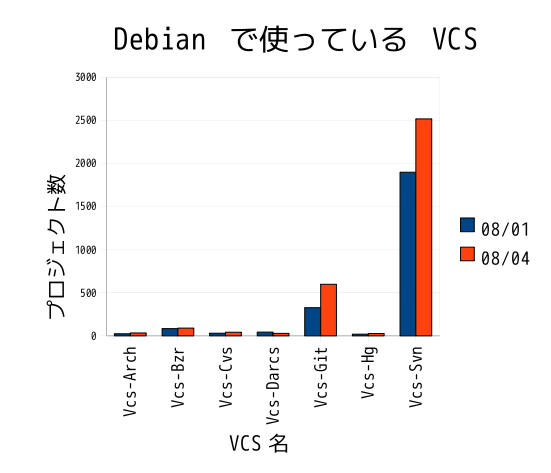
\includegraphics[width=0.5\hsize]{image200804/debian-vcs-200804.png}
\end{center}

\subsection{ソースパッケージを Git で管理するためのツール git-buildpackage}
\index{git-buildpackage} 
\index{git} 
では、実際に VCS を使って Debian Package を管理するためにはどのようにすればいいのでしょうか。
Debian パッケージを Git で管理するためのツールとして、 git-buildpackage があります。
これを使うことによって、Git を使ってパッケージのソースコードを管理することができるようになります。
インストールはいつものとおり、{\bf apt-get} or {\bf aptitude} を使ってインストールする
ことが可能です。

\begin{commandline}
$sudo apt-get install git-buildpackage
\end{commandline}

\subsubsection{git-buildpackageで提供されるコマンド}
git-buildpackageで提供されるコマンドは表\ref{git-buildpackage-command}の4つしかありません。
これらのコマンドと Git コマンド を使って、パッケージのメンテナンスをすることになります。
Gitの細かい知識は必要ありませんが、基本的な使い方は知っておく必要があります。
   \begin{table}[h]
    \begin{center}
      {
        \begin{tabular}{l|l} \hline
                提供されるコマンド & 機能 \\ \hline \hline
/usr/bin/git-buildpackage & パッケージを作成する \\
/usr/bin/git-dch & Git のコミットログから Debian Changelog を作成する。\\
/usr/bin/git-import-dsc & 既存の Debian Package をGitにインポートする。\\
/usr/bin/git-import-orig & アップストリームからリリースされたソースコードをGitにインポートする。\\
           \end{tabular}
        }
     \caption{git-buildpackage で提供されるコマンド}
     \label{git-buildpackage-command}
    \end{center}
    \end{table}

\subsection{Gitの簡単な使い方}
表\ref{git-command}によくつかう Gitコマンドを紹介します。これだけ知っていれば、Gitを使った開発を行う
ことが可能なはずです。
   \begin{table}[h]
    \begin{center}
      {
        \begin{tabular}{l|l} \hline
                Git コマンド(一部) & 機能 \\ \hline \hline
git init & ローカルリポジトリを作成する。\\
git add & ローカルリポジトリのキャッシュ(index)に管理対象のファイルを追加する。\\
git commit & ローカルリポジトリに変更を反映する。\\
git rm & ローカルリポジトリから管理対象ファイルを削除する。\\
git diff & 差分を取得する。\\
git branch & ブランチを作成する。\\
git checkout & 作成したブランチをチェックアウトする。\\
git format-patch & パッチを作成する。\\
           \end{tabular}
        }
     \caption{よく使うGitのコマンド}
     \label{git-command}
    \end{center}
    \end{table}

\subsection{既にパッケージ化されているものを Git で管理する}
Debian パッケージには2つの状態があると考えられます。一つは既にパッケージ化されているもの、
もうひとつは今からDebian パッケージにしようとしているものです。
まずは、既にDebian パッケージになっているものを Git で管理する方法を説明します。
\\

まず、git-import-dscコマンドを使い、 Git リポジトリに現在のソースコードの状態を
取り込みます。コマンドのオプションに、パッケージの dscファイル\footnote{Debian パッケージの制御ファイル}
を指定します。実行すると、パッケージ名でディレクトリが作成され、Git リポジトリが作成されます。
また、ブランチとして、master ブランチと、upstream ブランチが作成されます。 Debian 関係のコードは
 master 
ブランチ、Upstream のソースコードは upstream ブランチで管理されるようになります\footnote{ブランチは git branch コマンドで表示可能}。

\begin{commandline}
$ git-import-dsc ../isight-firmware-tools_1.0.2-1.dsc
Upstream version: 1.0.2
Debian version: 1
No git repository found, creating one.
Initialized empty Git repository in .git/
Everything imported under isight-firmware-tools
$ ls
isight-firmware-tools
$ cd isight-firmware-tools
$ git branch
* master
  upstream
\end{commandline}

\subsubsection{インポート時のログ}

パッケージをインポートしたときに、Git のコミットログに現在のバージョンのコミットログが書き込まれます。
また、 Debian Version は Git のタグ機能を使い、タグ名として保存されます。

\begin{commandline}
$ git log
commit 9c3669a233afe69d7be2aa8ad1995e6b19c841aa
Author: Nobuhiro Iwamatsu <iwamatsu@nigauri.org>
Date:   Sun Apr 6 21:48:40 2008 +0900

    Imported Debian patch 1.0.2-1
$ git tag
debian/1.0.2-1
upstream/1.0.2
\end{commandline}

\subsubsection{ソースコードを変更し、修正を管理する}

ソースコードを修正し、Debian Package で配布する部分を管理するには、今までどおり、dpatchなどの
パッチ管理システムを使う必要があります。
作成したパッチをリポジトリにコミットする時にに、{\bf git add}, {\bf git commit} コマンドを使い、
リポジトリに反映させます。

\begin{commandline}
$ dpatch-edit-patch 05_change_ift-load_install_dir
... いろいろ修正 ...
$ exit
$ vi debian/patches/00list
$ git add debian/patches/05chage_ift-load_install_dir.dpatch
$ git commit -s debian/patches/00list debian/patches/05_chage_ift-load_install_dir.dpatch
/* エディタが起動するので、コミットログを記述 */

Change ift-load install dir.
    
Signed-off-by: Nobuhiro Iwamatsu <iwamatsu@nigauri.org>

$ git log
commit c9865153ae1949956fdfe3827c0da9b36c2f0ddb
Author: Nobuhiro Iwamatsu <iwamatsu@nigauri.org>
Date:   Sun Apr 6 21:23:20 2008 +0900

    Change ift-load install dir.
    
    Signed-off-by: Nobuhiro Iwamatsu <iwamatsu@nigauri.org>
\end{commandline}

\subsubsection{git-buildpackage を使ったDebian パッケージの作成}

Debian パッケージを作成するには、 git-buildpackage コマンドを使います。
--git-ignore-new オプションは Git に反映されていない修正を無視するための
オプションです。
\begin{commandline}
$ git-buildpackage --git-ignore-new -us -uc
\end{commandline}

\subsubsection{パッケージをリリースする}
新しい Debian バージョンのパッケージをリリースする場合は、{\bf git-dch} コマンドに
{\bf --release} オプションを付けます。実行することにより、エディタが立ち上がり、Git
のコミットログから、Debian Changelog が作成されます。
Changelog を作成したら、{\bf git-buildpackage} コマンドに {\bf--git-tag} オプションを
付けてパッケージを作成します。{\bf--git-tag} を付けると、リポジトリに Debian バージョン用の
タグが Debian changelog より作成され、リリース情報が付加されます。
\begin{commandline}
$ git-dch --release
$ git-buildpackage --git-ignore-new --git-tag
$ git tag
debian/1.0.2-1
debian/1.0.2-2
upstream/1.0.2
\end{commandline}

\subsubsection{新しいバージョンにする}
新しいバージョンにするには、git-import-orig コマンドを使い、リリースされた
新しいバージョンの Tar ボールを指定します。
指定することにより、ファイル名からバージョンを取得し、新たにUpstream 用の
タグが作成されます。
また、アップストリームのバージョンが上がるため、自動的に Debian Changelog に 次のDebian Package 
バージョンが追記されます。
\begin{commandline}
$ git-import-orig /tmp/isight-firmware-tools-1.2.tar.gz
Upstream version is 1.2.0
Importing '/tmp/isight-firmware-tools-1.2.tar.gz' to branch 'upstream'...
Switched to branch "upstream"
rm 'isight.rules.in'
rm 'po/fr_FR.po'
Created commit f5c85da: Imported Upstream version 1.2.0
 33 files changed, 4434 insertions(+), 1332 deletions(-)

.......<snip>

 src/udev.c                             |  164 +++
 33 files changed, 4434 insertions(+), 1332 deletions(-)
 rename po/{fr_FR.po => fr.po} (66%)
 create mode 100644 src/50-isight-firmware.fdi
 create mode 100644 src/callout.c
 create mode 100644 src/isight-firmware.fdi
 rename isight.rules.in => src/isight.rules.in (100%)
 create mode 100644 src/load.h
 create mode 100644 src/udev.c
Succesfully merged version 1.2 of /home/iwamatsu/Desktop/isight-firmware-tools-1.2.tar.gz into .
$ git branch
debian/1.0.2-1
debian/1.0.2-2
upstream/1.0.2
upstream/1.2
$ cat debian/changelog
isight-firmware-tools (1.2-1) unstable; urgency=low

  * New Upstream Version

 -- Nobuhiro Iwamatsu <iwamatsu@nigauri.org>  Fri, 11 Apr 2008 17:18:23 +0900

\end{commandline}

\subsection{新たにパッケージ化する場合}
あたらしくにソフトウェアを Debian Package にして、 git-buildpackage で
管理する場合は 最初に Git の機能が必要です。
まず、ローカル Git リポジトリを作成します。次に作成したリポジトリに移動し、{\bf git-import-orig}
コマンドにアップストリームのソースコードを指定し、実行します。ソースコードは、gzip、bzip2 などで
圧縮されたものと、展開されたソースコードディレクトリを指定することが可能です。
また、実行する際に、{\bf-u} オプションで、アップストリームのバージョンを指定する事が可能です。
リポジトリを作成した後は upstream ブランチに移動し、{\bf dh\_make}等を使ってパッケージの雛形作成し、
上で説明した流れでメンテナンスを行います。

\begin{commandline}
$ mkdir isight-firmware-loader-1.2
$ cd isight-firmware-tools-1.2
$ git init /* ローカル Git リポジトリを作成する */
$ git-import-orig -u 1.2  /tmp/isight-firmware-tools-1.2.tar.gz /* ソースコードをコミット */
Upstream version is 1.2
Initial import of '/tmp/isight-firmware-tools-1.2.tar.gz' ...
Succesfully merged version 1.2 of /tmp/isight-firmware-tools-1.2.tar.gz into .
$ git log
commit 9bf014aee2f834576f8f03d67ab66e8c85726832
Author: Nobuhiro Iwamatsu <iwamatsu@nigauri.org>
Date:   Tue Apr 8 21:42:55 2008 +0900

    Imported Upstream version 1.2
$ git branch
* master
  upstream
$ git tag
upstream/1.2
$ git branch upsteam
$ dh_make
$ git branch master
\end{commandline}

%\subsubsection{git-buildpackage の設定 .git/gbp.conf}
%git-buildpackage は細かい設定を行うことが可能です。
%設定ファイルを .git ファイル


\dancersection{アップストリームの VCS と付き合う}{岩松 信洋}
\label{sec:upstreamvcs}
\index{DebianWithVCS}
% CVS / SVN / Git などの VCS をupstream が活用している場合の話。

VCS を使ってアップストリームがソフトウェアの開発を行っている事が多くあります。
アップストリームでは、Subversion を使っているが、パッケージメンテナは Git を使って
パッケージを行っている場合があったり、同じ VCS を使っている場合もあります。
今回は  Subversion を例にして、お互い VCS を使っている場合、どのように付き合って
いくことができるのか説明します。

%\subsection{アップストリームが Git を使っている場合 }
%\subsection{アップストリームが CVS を使っている場合 }

\subsection{アップストリームが Subversion を使っている場合 }
Subversion で管理されているソースコードを取得したり、Subversion リポジトリへ
コミットするツールとして、git-svn パッケージがあります。 git-svn を使うことに
よって、容易に お互いのリポジトリ間を行き来することができるようになります。

\subsubsection{Subversion のリポジトリから Git のリポジトリへ ソースコードを取得する}
Subversion のリポジトリから Git のリポジトリへ ソースコードを取得するには
適当なディレクトリを作成し、 {\bf git svn} の {\bf clone} オプションを使って行います。 
取得した後は、Git の操作で開発を行うことができます。

\begin{commandline}
$ mkdir test
$ git svn clone svn://test/trunk test-0.0.1
\end{commandline}

\subsection{取得したコードを元に Debian Package を作成する}
取得したコードから新しく Debian Package を作成するためには、自分でタグを付ける必要があります。
{\bf git-buildpackage}ではタグと Debian changelog から Upstream の情報を取得し、
orig.tar.gz 相当のものを作成するため、タグを付ける必要があります。

\begin{commandline}
$ git branch
master
$ git branch upstream
$ git checkout upstream
$ git tag upstream/0.0.1
$ dh_make --createorig
$ git branch master
.... Debian Package 用のファイル作成などを行う ....
$ git-buildpackage -us -uc --git-ignore-new
$ debuild clean
$ git add debian
$ git commit -a
$ git-buildpackage -us -uc --git-ignore-new --git-tag
\end{commandline}


\subsubsection{Subversion リポジトリの情報を取得する}
Subversion リポジトリの情報を取得するには、 {\bf rebase}オプションを使います。
最初から git svn でリポジトリの操作を行っている場合は、rebase を使うことにより、
Upstream のコードを パッケージ側に反映させることができます。
\begin{commandline}
$ git checkout upstream
$ git svn rebase
\end{commandline}

\subsection{すでにあるパッケージと Git リポジトリを元に Debian Package を作成する}

\begin{minipage}{0.5\hsize}
{\bf git svn} で取得した Git リポジトリと 既にあるDebian Package を連携させるには
操作が少し必要です。
まず、{\bf git-import-dsc} で 現在の Debian Package を git-buildpackage で管理できる
ようにした後、upstream ブランチに git svn で取得したリポジトリから pull をします。
pull することにより、コミットログの共有することができます。
しかし、Debian Changelog の操作や、{\bf git tag} を使ったタグの操作を手動で行う必要がある
のが問題点です。
{\bf git-import-org } を使って、tar.gz や ソースコードを指定して、マージすることも可能ですが、
Upstream 側のコミットログが取り込まれないため、 Gitを使うメリットがあまり無いと私は考えています。
このあたりを改善していく事が今後の課題になりそうです。
\end{minipage}
\begin{minipage}{0.5\hsize}
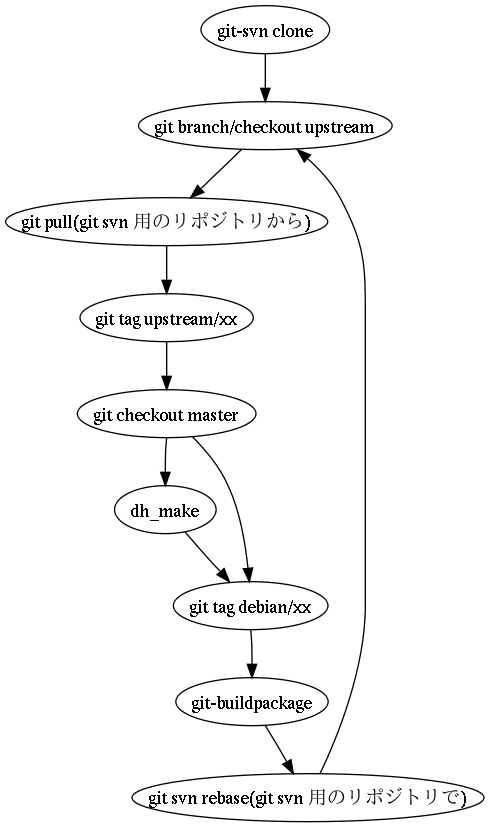
\includegraphics[width=0.8\hsize]{image200804/git-svn_with_build-package.png}
\end{minipage}

\begin{commandline}
$ git svn clone svn://svn.berlios.de/linux-uvc/linux-uvc/trunk\
 linux-uvc.git
$ git import-dsc  ../../../debian/linux-uvc_0.1.0.svn193-2.dsc
$ cd linux-uvc
$ git branch
* master
  upstream
$ git tag
debian/0.1.0.svn193-2
upstream/0.1.0.svn193
$ git checkout upstream
$ git pull ../linux-uvc.git/
$ git tag upstream/0.1.0.svn201
$ git checkout master
$ dch -v 0.1.0.svn201
$ git-buildpackage -us -uc --git-ignore-new
$ debuild clean
$ git commit -a
$ git-buildpackage -us -uc --git-ignore-new --git-tag
\end{commandline}

\dancersection{Nexenta Core Platformを使ってみる}{上川 純一}
\label{sec:nexentacore}
\index{OpenSolaris} 
\index{Nexenta} 

\subsection{はじめに}

Nexenta\footnote{\url{http://www.nexenta.org/os}}とは Debian GNU/Linux のパッケージングシステムを OpenSolaris\footnote{\url{http://www.opensolaris.org/os/}}に移
植したもののようです。OpenSolaris とは Solarisのオープンソース版のようで
す。Nexenta Core Platform が2008年2月にリリースされました。今回はそれを試
してみます。

\subsection{ダウンロード}

\url{http://www.nexenta.org/os/DownloadMirrors}からリンクをたどりダウン
ロードします。
今回は
\url{http://mirror.stanford.edu/nexenta/isos/nexenta-core-platform_1.0-b82_x86.iso.zip}
を利用しました。

unzipコマンドで展開するとisoイメージが作成されます。
\begin{commandline}
[21:54:42]dancer64:nexenta> unzip nexenta-core-platform_1.0-b82_x86.iso.zip 
Archive:  nexenta-core-platform_1.0-b82_x86.iso.zip
  inflating: nexenta-core-platform_1.0-b82_x86.iso  
\end{commandline}

\subsection{Qemu環境でのインストール}

まず、qemu 用のディスクイメージを作成します。
\begin{commandline}
$ qemu-img create -f qcow2 nexenta.cow 3GB 
Formatting 'nexenta.cow', fmt=qcow2, size=3145728 kB
\end{commandline}

qemuを起動します。
\footnote{時間の設定についてはただしい組み合わせを見つけられませんでした。
BIOS時間をローカルタイムとして扱うわけでもなく、UTCとして扱うわけでもな
いように見えます。正しい設定をご存知でしたらご一報ください。}

\begin{commandline}
$ qemu-system-x86_64 -hda nexenta.cow \
 -cdrom  nexenta-core-platform_1.0-b82_x86.iso \
 -boot d \
 -m 512 
\end{commandline}


メニューを選択し順番にインストール作業を進めます。

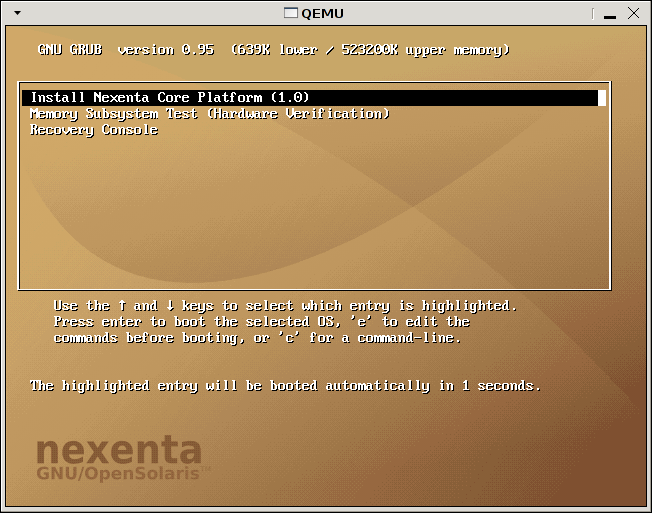
\includegraphics[width=0.5\hsize]{image200804/nexenta1.png}
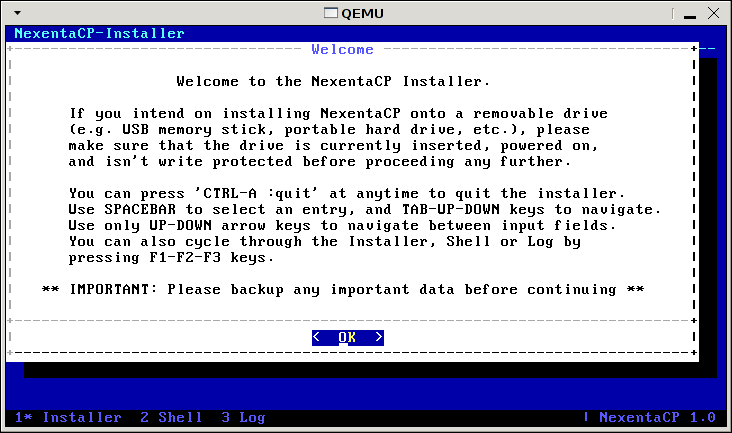
\includegraphics[width=0.5\hsize]{image200804/nexenta2.png}
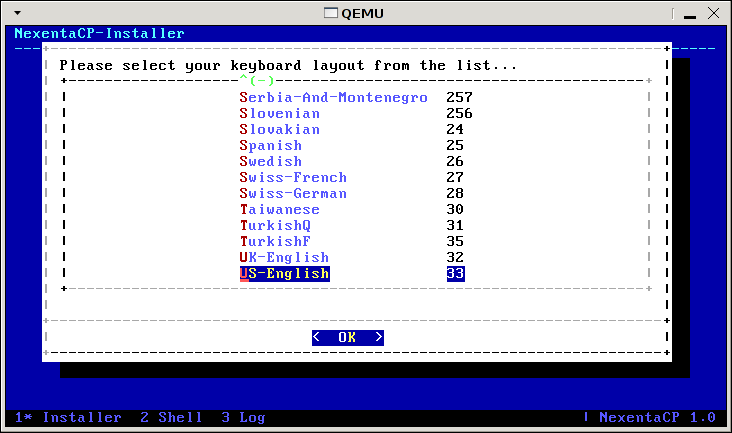
\includegraphics[width=0.5\hsize]{image200804/nexenta3.png}
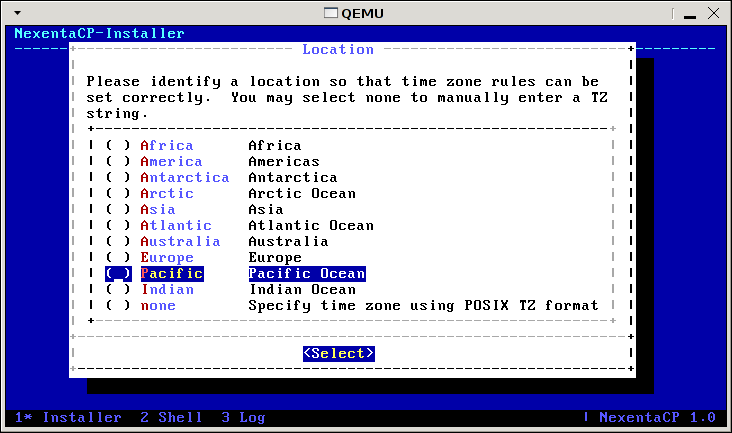
\includegraphics[width=0.5\hsize]{image200804/nexenta4.png}
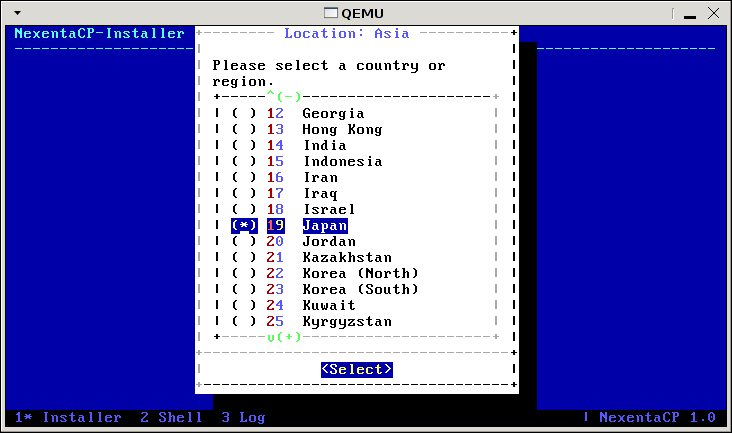
\includegraphics[width=0.5\hsize]{image200804/nexenta5.png}
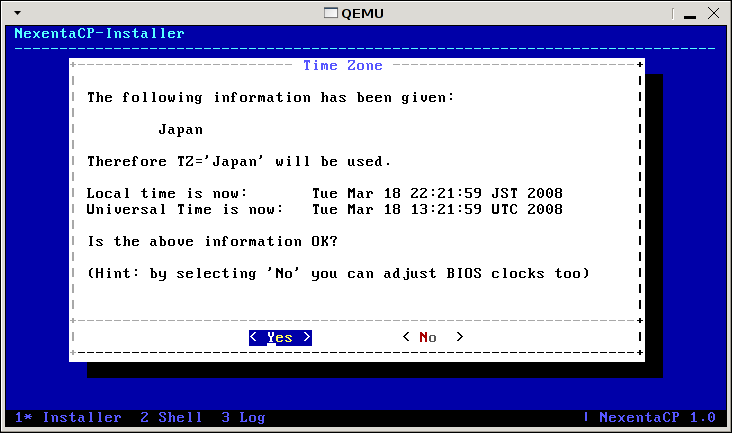
\includegraphics[width=0.5\hsize]{image200804/nexenta6.png}
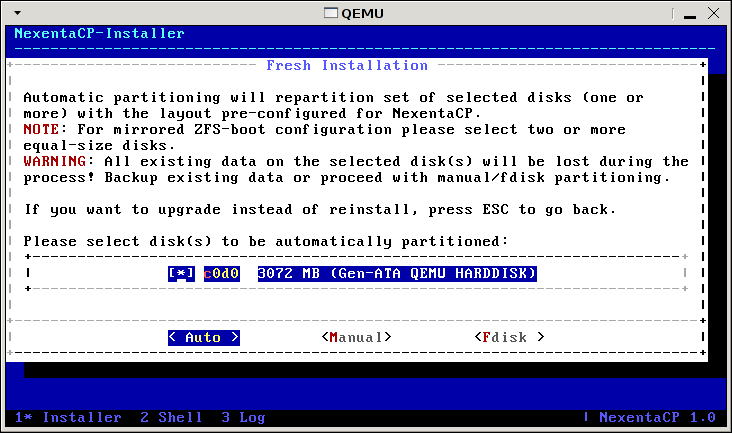
\includegraphics[width=0.5\hsize]{image200804/nexenta7.png}
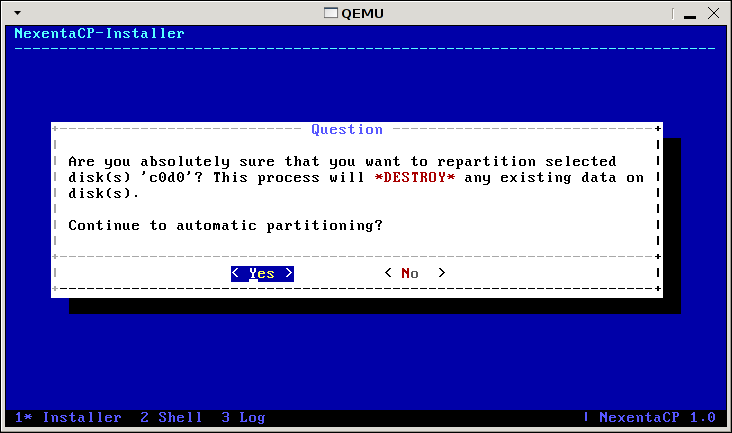
\includegraphics[width=0.5\hsize]{image200804/nexenta8.png}

インストールが開始したらしばし待ちます。\footnote{AMD Athlon 64 3500+ の
マシン(64bit)でkqemuを利用して2時間かかりました}

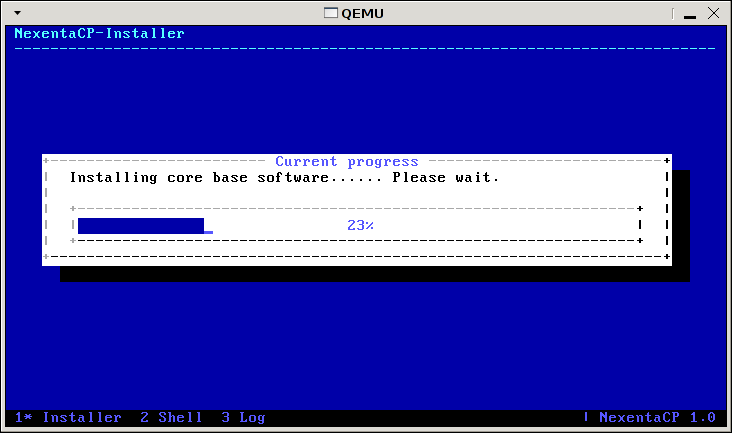
\includegraphics[width=0.5\hsize]{image200804/nexenta9.png}
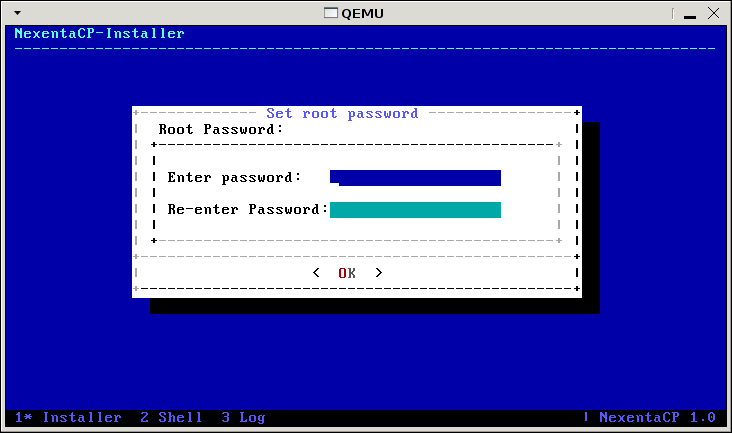
\includegraphics[width=0.5\hsize]{image200804/nexenta10.png}
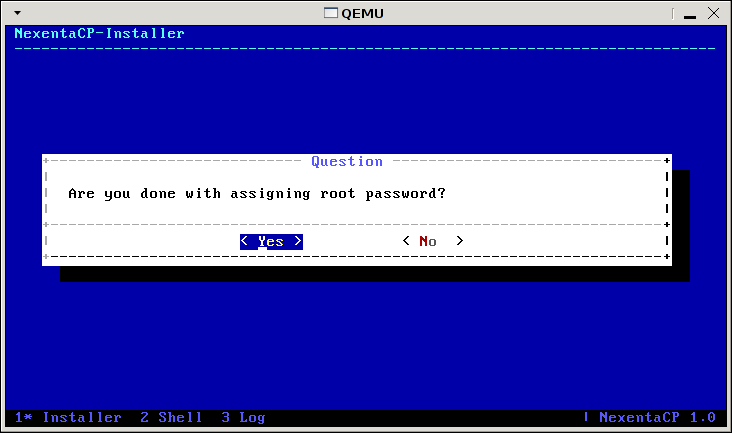
\includegraphics[width=0.5\hsize]{image200804/nexenta11.png}
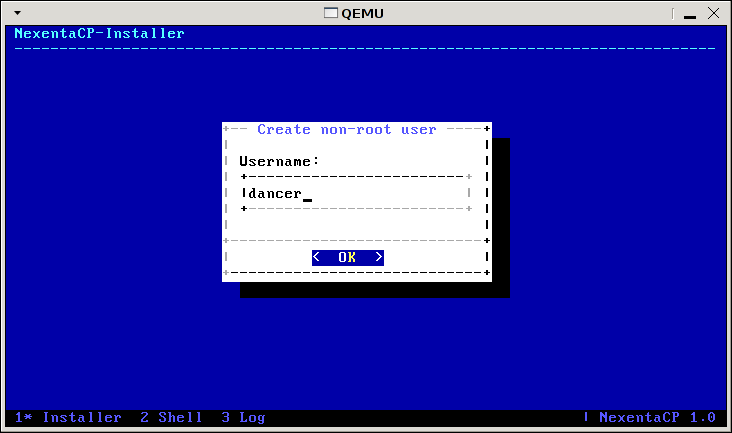
\includegraphics[width=0.5\hsize]{image200804/nexenta12.png}
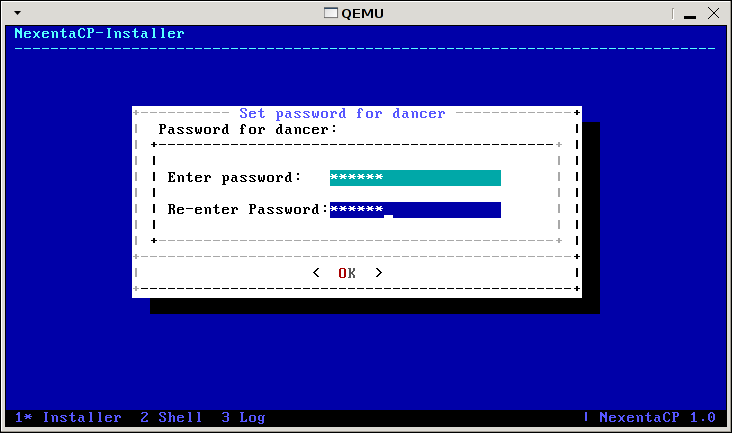
\includegraphics[width=0.5\hsize]{image200804/nexenta13.png}
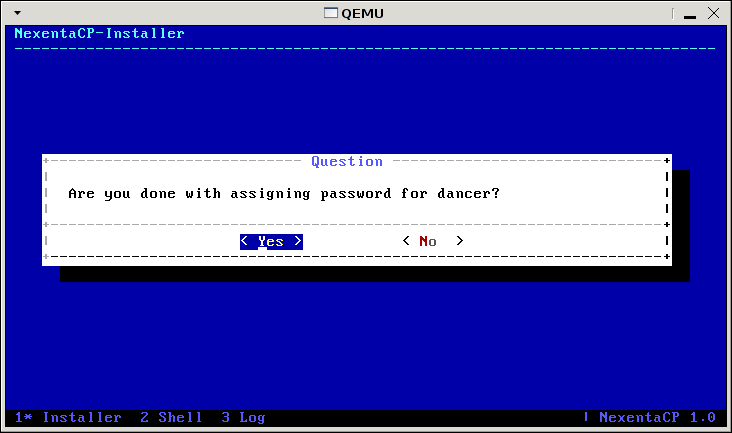
\includegraphics[width=0.5\hsize]{image200804/nexenta14.png}
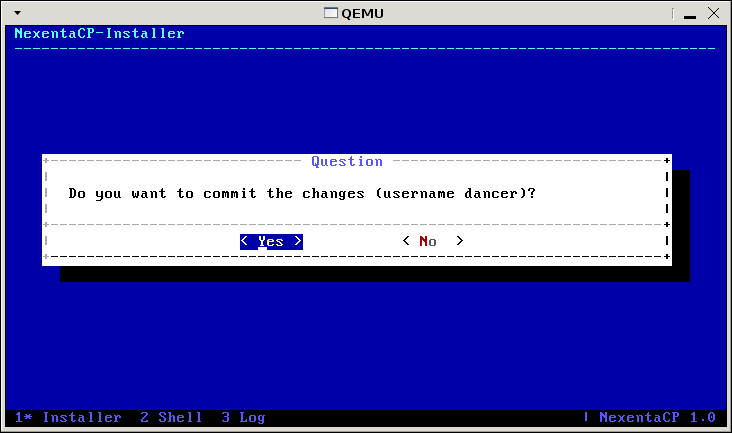
\includegraphics[width=0.5\hsize]{image200804/nexenta15.png}
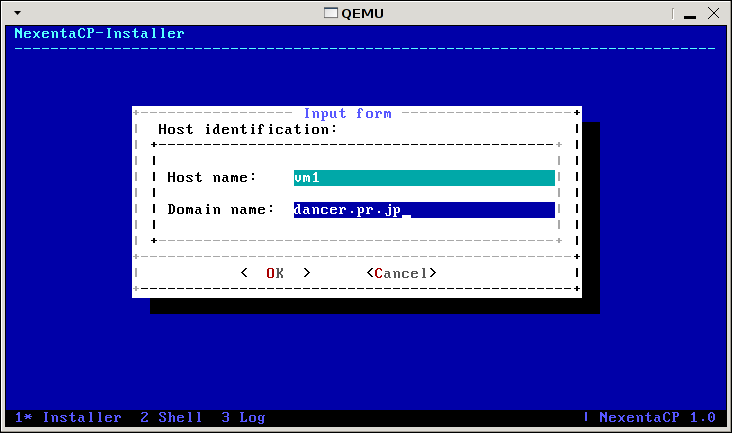
\includegraphics[width=0.5\hsize]{image200804/nexenta16.png}
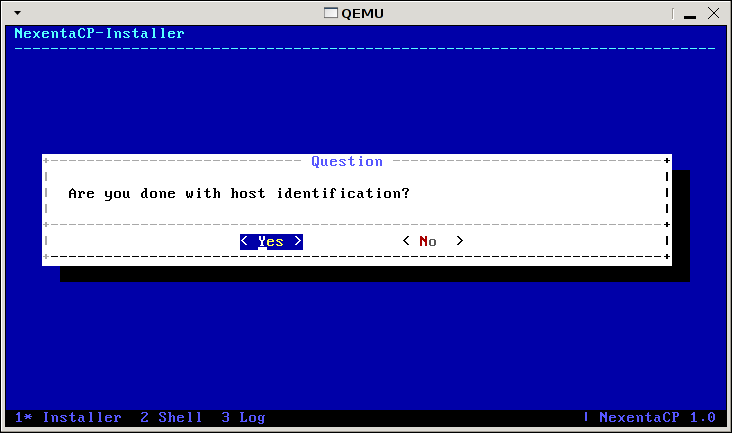
\includegraphics[width=0.5\hsize]{image200804/nexenta17.png}
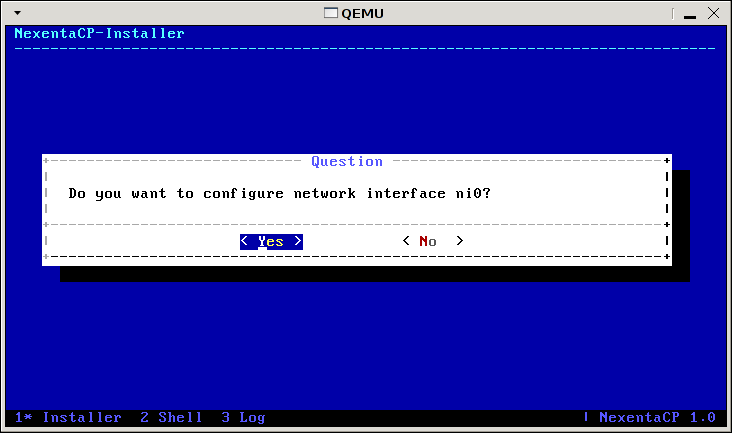
\includegraphics[width=0.5\hsize]{image200804/nexenta18.png}
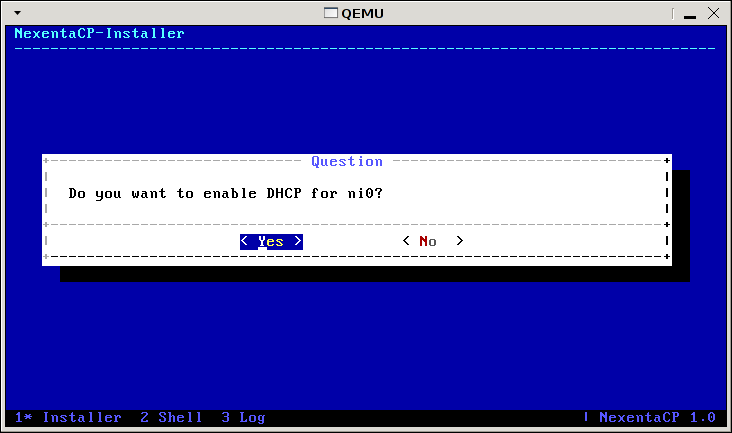
\includegraphics[width=0.5\hsize]{image200804/nexenta19.png}
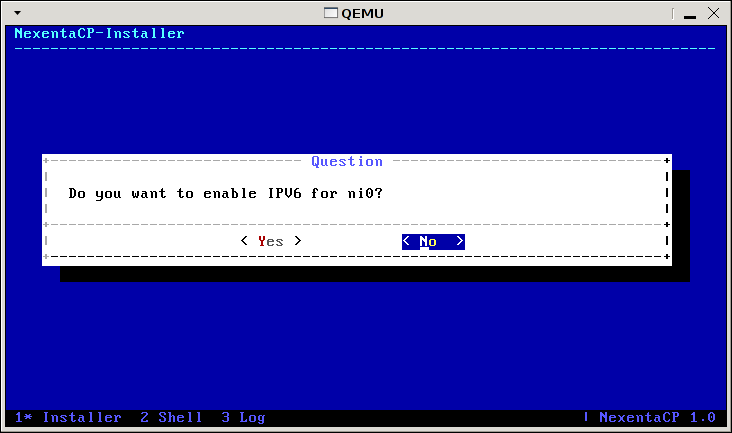
\includegraphics[width=0.5\hsize]{image200804/nexenta20.png}
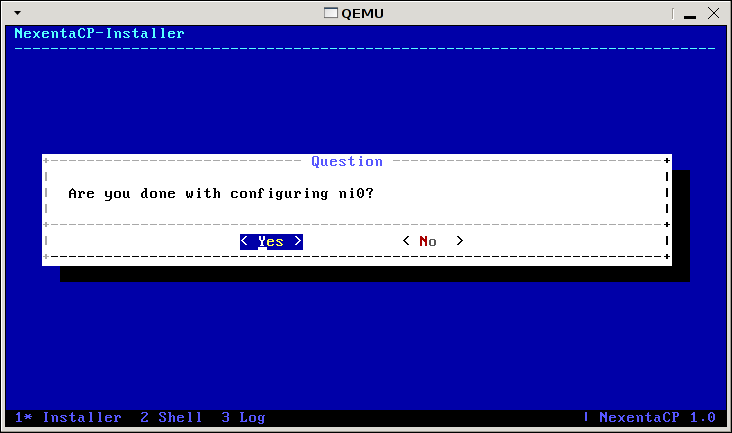
\includegraphics[width=0.5\hsize]{image200804/nexenta21.png}
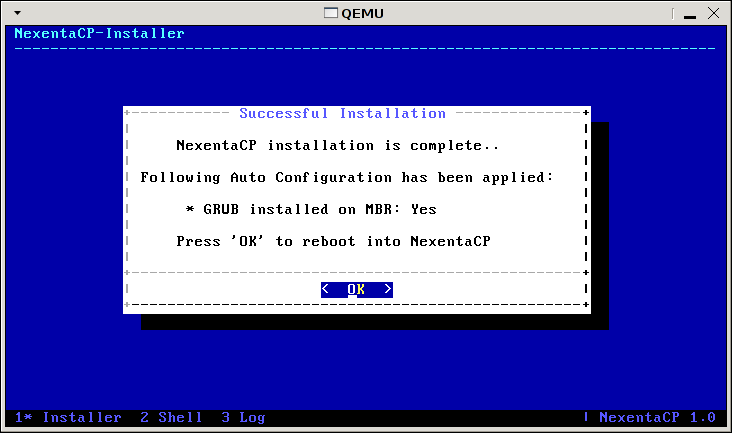
\includegraphics[width=0.5\hsize]{image200804/nexenta22.png}

\subsection{実行してみる}

それでは、インストールしたOSを起動してみましょう。メモリは512MB程度割り
当てないと起動しないようです。

\begin{commandline}
$ qemu-system-x86_64 -hda nexenta.cow \
 -m 512 -kernel-kqemu \
 -redir tcp:2222::22
\end{commandline}

手元のシステムでは、コマンドラインでログインができる状態まで3分程度かかりました。

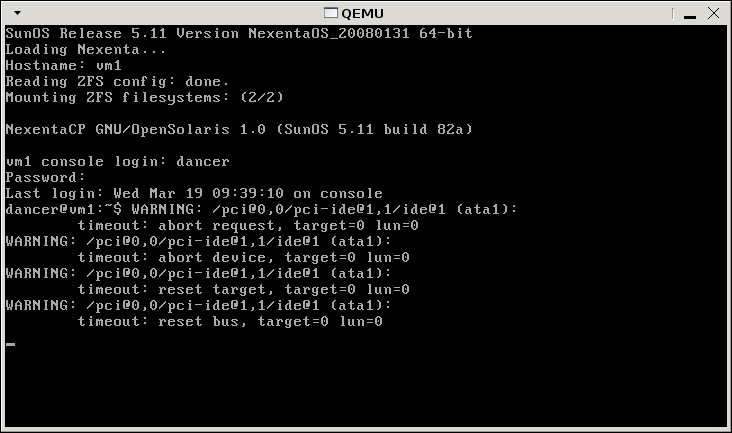
\includegraphics[width=0.5\hsize]{image200804/nexenta23.png}

通常のコンソールのログイン画面が立ち上がり、ログイン可能になります。

デフォルトで sshd \footnote{Debian のパッケージとは異なり、SUNWsshdu,
SUNWsshdr などのパッケージになっています。見た感じは alien で作成されてい
るパッケージのようです。} などもインストールされているようです。
netstat で確認するとlisten しているようですので、ssh でログインして作業
することが可能なようです。
ここでは、 qemu で -redir オプションを使い、 SSHの22番ポートをホストOSの
2222ポートからアクセスできるようにしています。

-nographic -serial stdio オプションも追加してヘッドレスで稼働させることも
可能です。ただし、デフォルトではシリアルコンソールには何も出力されないようです。

ネットワークデバイスは ni0 になっているようです。IPアドレスは qemu の機
能で DHCPで提供されているアドレス(10.0.2.15)になっています。


\subsection{Debian との互換性}

初期インストールのパッケージ数が非常に多いです。OpenSolaris のデフォルト
インストールに相当するものをそのままパッケージにしているのでしょうか?
SUNWではじまるパッケージ名などがそれっぽさを物語ります。

\begin{commandline}
dancer@vm1:~$ dpkg -l | wc -l 
464
dancer@vm1:~$ dpkg -l 
Desired=Unknown/Install/Remove/Purge/Hold
| Status=Not/Installed/Config-files/Unpacked/Failed-config/Half-installed
|/ Err?=(none)/Hold/Reinst-required/X=both-problems (Status,Err: uppercase=bad)
||/ Name           Version        Description
+++-==============-==============-============================================
ii  adduser        3.80nexenta3   Add and remove users and groups
ii  alien          8.73.4         install non-native packages with dpkg
ii  apt            0.6.46.4nexent Advanced front-end for dpkg
ii  apt-utils      0.6.46.4nexent APT utility programs
ii  aptitude       0.4.4-1nexenta terminal-based apt frontend
[中略]
ii  sunw1394       5.11.82-1      Sun IEEE1394 Framework
ii  sunwaac        5.11.82-1      Adaptec AdvanceRaid Controller SCSI HBA Driv
ii  sunwad810      5.11.82-1      SUNW W1100z & W2100z Audio Drivers
ii  sunwadixp      5.11.82-1      SUNW Audio Driver for ATI IXP
ii  sunwadpu320    5.11.82-1      Adaptec Ultra320 Driver
ii  sunwafe        5.11.82-1      ADMtek Ethernet Driver
ii  sunwagp        5.11.82-1      AGP GART Driver
ii  sunwahci       5.11.82-1      Advanced Host Controller Interface (AHCI) SA
ii  sunwamd8111s   5.11.82-1      AMD8111 FAST Ethernet Network Adapter Driver
ii  sunwamr        5.11.82-1      LSI MegaRAID SCSI HBA Driver
[中略]
ii  sunwsshcu      5.11.82-1      SSH Common, (Usr)
ii  sunwsshdr      5.11.82-1      SSH Server, (Root)
ii  sunwsshdu      5.11.82-1      SSH Server, (Usr)
ii  sunwsshr       5.11.82-1      SSH Client and utilities, (Root)
ii  sunwsshu       5.11.82-1      SSH Client and utilities, (Usr)
ii  sunwtavor      5.11.82-1      Sun Tavor HCA driver
[略]
\end{commandline}

\subsection{ないパッケージをビルドしてみた}

/etc/hostsをいじってみようとしたら、シンボリックリンクになってました。し
かも root 権限でも書き込み不可になっています。

\begin{commandline}
root@vm1:/export/home/dancer# ls -l /etc/hosts
lrwxrwxrwx 1 root root 12 Mar 19 08:15 /etc/hosts -> ./inet/hosts
root@vm1:/export/home/dancer# ls -l /etc/inet/hosts -l 
-r--r--r-- 1 root sys 1078 Apr  6 10:28 /etc/inet/hosts
\end{commandline}

気をとりなおして、 /etc/apt/sources.list に適当にソースを追加します。

\begin{commandline}
deb-src http://cdn.debian.or.jp/debian unstable main contrib non-free
\end{commandline}

apt-listbugs が存在しないみたいなので、ビルドしてみようと思います。

まず、なぜだか racc, rdtool が足りないのでビルドしてインストールします。
無事にapt-listbugs 自体もビルドできたので、意気揚々とインストールしてみま
す。

\begin{commandline}
root@vm1:/tmp/apt-listbugs-0.0.88# debi
Selecting previously deselected package apt-listbugs.
(Reading database ... 27441 files and directories currently installed.)
Unpacking apt-listbugs (from apt-listbugs_0.0.88_all.deb) ...
dpkg: dependency problems prevent configuration of apt-listbugs:
 apt-listbugs depends on ruby (>= 1.8); however:
  Package ruby is not installed.
 apt-listbugs depends on libruby1.8 (>= 1.8.5); however:
  Version of libruby1.8 on system is 1.8.4-1nexenta1.3.
 apt-listbugs depends on libdpkg-ruby1.8 (>= 0.3.2); however:
  Package libdpkg-ruby1.8 is not installed.
 apt-listbugs depends on libgettext-ruby1.8; however:
  Package libgettext-ruby1.8 is not installed.
 apt-listbugs depends on libxml-parser-ruby1.8; however:
  Package libxml-parser-ruby1.8 is not installed.
 apt-listbugs depends on libhttp-access2-ruby1.8 (>= 2.0.6); however:
  Package libhttp-access2-ruby1.8 is not installed.
dpkg: error processing apt-listbugs (--install):
 dependency problems - leaving unconfigured
Errors were encountered while processing:
 apt-listbugs
debi: debpkg -i failed
\end{commandline}

残念、いくつかエラーがあるようです。ruby 自体が古いというエラーや、いくつ
かのライブラリが足りないというエラーがでています。

解決できそうな問題も、解決できなさそうな問題もあります。先は長いか?

\subsection{まとめ}

今回はNexenta Core Platformをとりあえず仮想マシンにインストールしてみまし
た。いろいろとDebian GNU/Linuxと違う部分があったので、今後どのように開発
がすすむのか、気になります。

\clearpage

%\printindex

\cleartooddpage

\vspace*{15cm}
\hrule
\vspace{2mm}

\includegraphics[width=2cm]{image200502/openlogo-nd.eps}
\noindent \Large \bf Debian 勉強会資料\\ \\
\noindent \normalfont \debmtgyear{}年\debmtgmonth{}月\debmtgdate{}日 \hspace{5mm}  初版第1刷発行\\
\noindent \normalfont 東京エリア Debian 勉強会 (編集・印刷・発行)\\
\hrule


\end{document}
